\section{Použité metatechnologie}
\label{sec:used-metatechnologies}

\subsection{Git}
\label{subsec:git}

\begin{wrapfigure}{R}{.5\textwidth}
 \centering
 \includesvg[width=.5\textwidth]{assets/git-logo}
 \caption{Logo verzovacího systému Git}
\end{wrapfigure}

Git je distribuovaný systém správy verzí, původně určený pro vývoj jádra Linuxu. Jako jeho autor je označován Linus Torvalds\cite{git-docs}, jeho vznik se datuje kolem 2005 a v~roce 2016 je nadále aktivně vyvíjen; jeho poslední verze nese označení 2.7.3 a byla vydána 10. března 2016. Nejčastěji slouží k~verzování zdrojového kódu - vytváří historii pro každou část spravovaného repozitáře.

Repozitář je v~tomto systému základní nejvyšší jednotka pro správu zdrojového kódu, zapouzdřuje jednotlivé vývojové větvě, ve kterých může probíhat vývoj od jednotlivých vývojářů zcela odděleně. Git je oproti jiným verzovacím nástrojům velmi silný v~následném spojování těchto větví - v~případě nekonfliktních změn je toto spojení schopen provést zcela sám, v~případě těch konfliktních zvládne označit konfliktní místa - pro následné vyřešení konfliktů stačí vyřešit konflikty přímo ve zdrojových souborech, avšak existují i grafická rozhraní. Schéma základních operací je možno pochopit z~obrázku\fullref{fig:git-operations}.

\begin{figure}[H]
 	\centering
 	\includesvg[width=.9\textwidth]{assets/git-operations}
 	\caption[Základní operace při práci se systémem Git]{Základní operace při práci se systémem Git\cite{basic-git-svg}}
 	\label{fig:git-operations}
\end{figure}

Git je plně ovladatelný z~příkazové řádky, avšak existuje velké množství jeho grafických nadstaveb, například jednoduchý \href{http://git-cola.github.io/}{git-cola} (náhled v~obrázku\fullref{fig:git-cola}) nebo o~mnoho komplexnější \href{https://www.sourcetreeapp.com/}{SourceTree}.

\begin{figure}[H]
	\centering
	% \begin{minipage}{.475\textwidth}
 % 		\centering
 % 		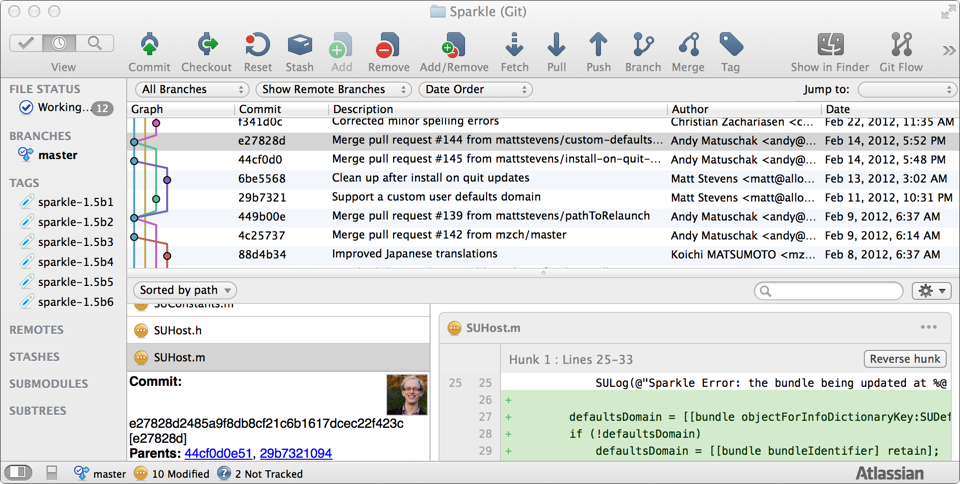
\includegraphics[width=\textwidth]{assets/source-tree-screenshot}
 % 		\caption{Screenshot z programu SourceTree}
	% \end{minipage}
	\begin{minipage}{.9\textwidth}
 		\centering
 		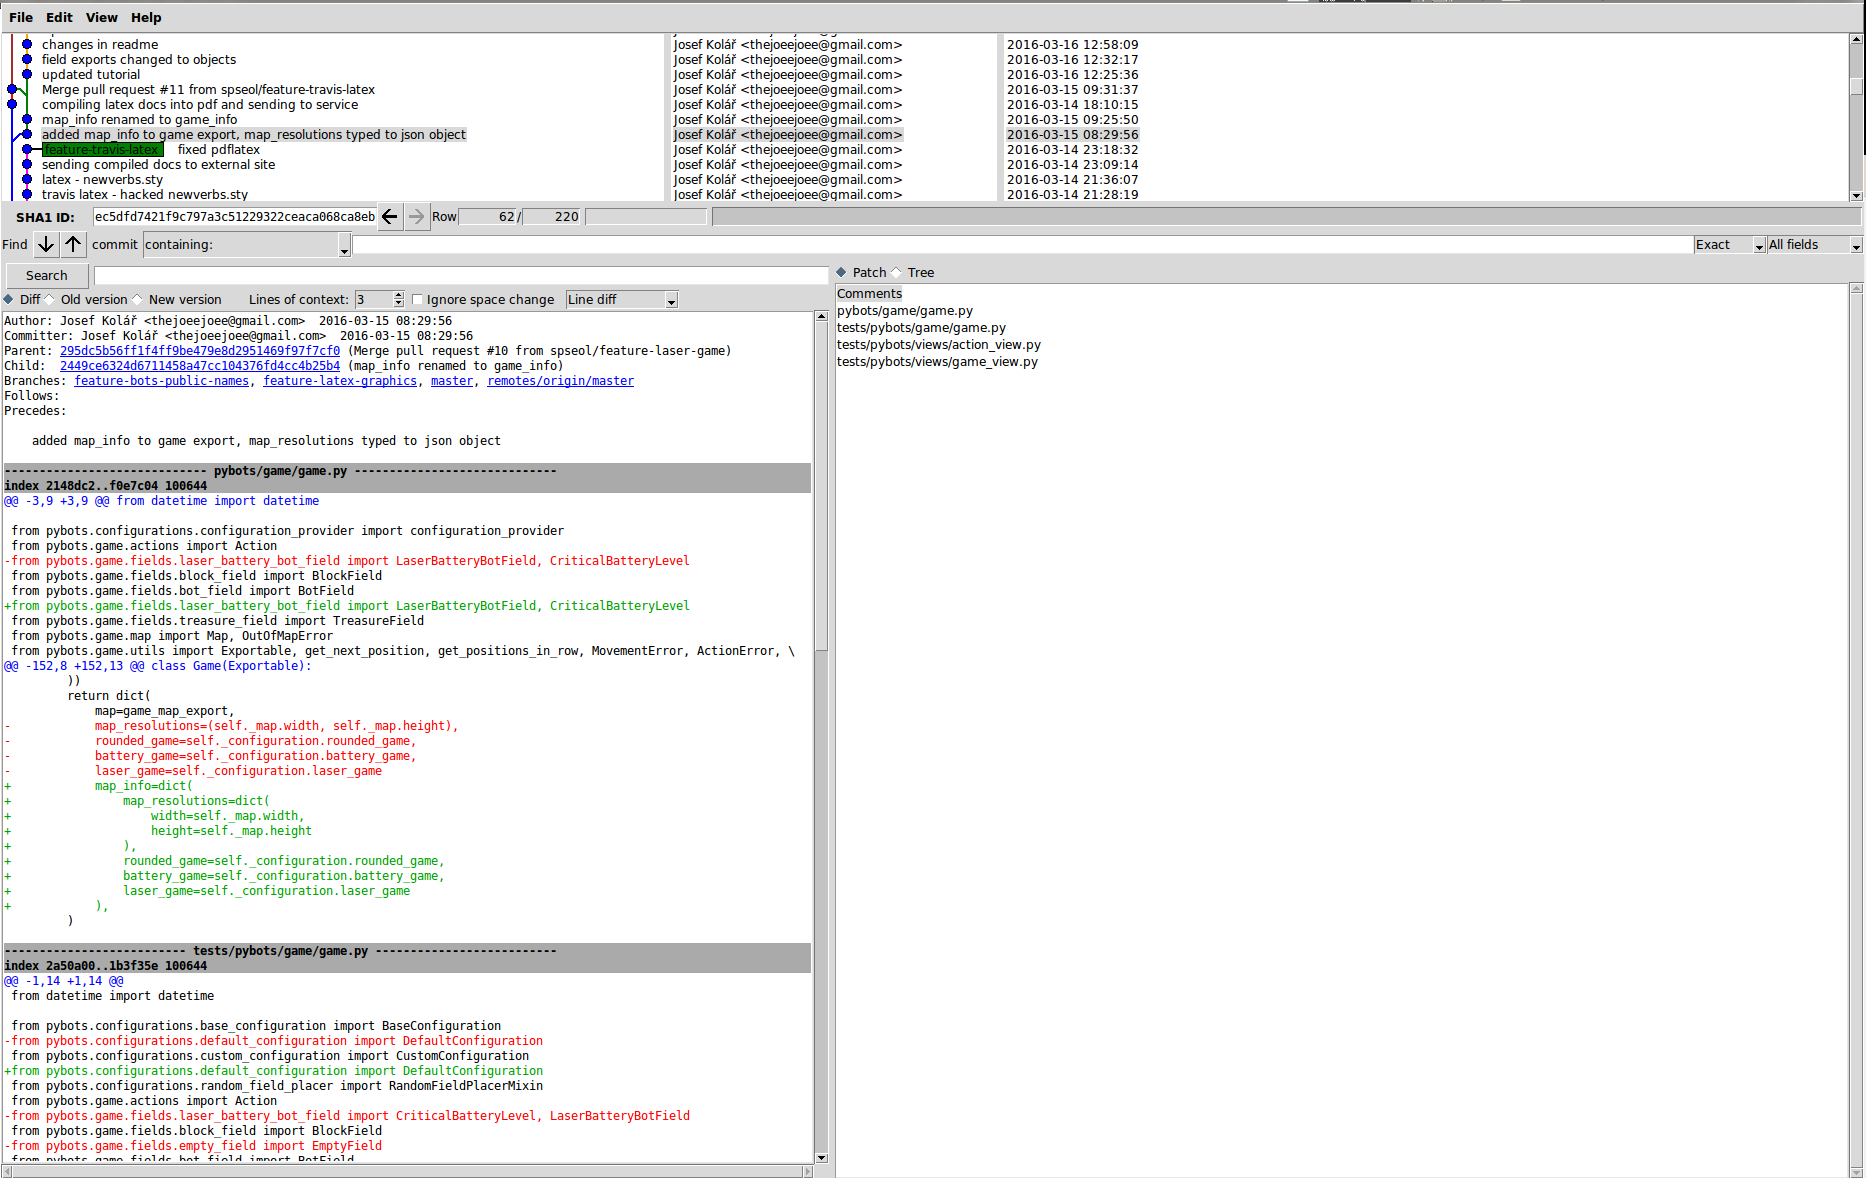
\includegraphics[width=.9\textwidth]{assets/git-cola-screenshot}
 		\caption{Screenshot z~programu git-cola}
 		\label{fig:git-cola}
 	\end{minipage}
\end{figure}

\subsection{GitHub}

\begin{wrapfigure}[18]{R}{.4\textwidth}
 	\centering
 	\includesvg[width=.4\textwidth]{assets/github-logo}
 	\caption{Logo systému pro správu git repozitářů GitHub}
\end{wrapfigure}

GitHub je webová služba poskytující podporu pro hostování \nameref{subsec:git} repozitářů. Pro veřejné repozitáře je tato služba zcela zdarma, pro soukromé repozitáře je zpoplatněna\cite{github-docs}. Kromě hostování nabízí i širokou škálu služeb týkajících se zdrojového kódu, jako například komentování zdrojového k\'{o}du, komentování jeho změn, systém úkolů, soukromých zpráv mezi vývojáři nebo možnost zařazení repozitáře mezi oblíbené. GitHub spustili v~roce 2008 vývojáři Tom Preston-Werner, Chris Wanstrath a PJ Hyett a nabízí i možnost napojení na jiné systémy, jako je například \nameref{subsec:travis-ci}. GitHub umí na základně uživatelských akcí (\ic|git push|, \ic|git pull|, \ic|git clone| a další) notifikovat externí služby pomocí HTTP POST požadavku na specifikovanou URL adresu - tato vlastnost se nazývá \uv{webhooks}. Repozitář tohoto projektu je také uložen na GitHubu pro adresou \url{https://github.com/spseol/pybots-server}.

\subsection{Travis CI}
\label{subsec:travis-ci}

Travis CI je webová služba zajišťující automatické sestavení a otestování změn zdrojového kódu v~repozitáři na GitHubu. Je řízen souborem \ic|.travis.yml|\cite{travis-docs}, ve kterém jsou definovány příkazy pro instalaci a nastavení prostředí a následné sestavení a spuštění testů projektu. Travis CI je specifický v~tom, že pro každé sestavení (\uv{build}) je rozběhnut samostatný kontejner s~nainstalovaným virtuální systémem. V~době psaní této práce je to distribuce \ic|Ubuntu 12.04.5 LTS|. 

\begin{wrapfigure}[16]{R}{.4\textwidth}
	\centering
	\includesvg[width=.4\textwidth]{assets/travis-logo}
	\caption{Logo automatického sestavovacího nástroje Travis CI}
\end{wrapfigure}

Při instalaci je možnost používat tradiční příkazy zapsané jazyce \ic|bash|, který tato distribuce používá jako výchozí příkazový interpret. \fullref{lst:travis-yml} také ukazuje možnost testovat projekt nad více verzemi Pythonu, v~mém případě je to \ic|Python 3.5.0|, \ic|Python 3.4.2|, \ic|PyPy 2.4.0 [Python 3.2.5]| (\href{http://pypy.org/}{interpret} Pythonu napsaný v~Pythonu) a \ic|nightly|, což je poslední vydaná verze Pythonu, aktuálně se jedná o~\ic|Python 3.6.0a0|. Detaily a historii sestavování jednotlivých změn zdrojového kódu lze zhlédnout na adrese \url{https://travis-ci.org/spseol/pybots-server}.

V~ukázce lze vidět také příkazy spouštěné při běhu kontejneru (\ic|install|, \ic|before_script|, \ic|script| a \ic|after_success|), ve kterých se postupně nejprve nainstalují Python závislosti ze souboru \ic|requirements.txt|, poté zaznamenávač pokrytí kódu \ic|coverage| a poté linter \ic|pep8|, který následně zkontroluje zdrojový kód a v~případě úspěchu se na řádku $17$ spustí samotné testy. Celý běh je zakončen odesláním výsledků pokrytí na službu \href{https://coveralls.io/}{coveralls.io}. V~sekcích \ic|language|, \ic|python| a \ic|matrix| je uložena konfigurace pro různé verze jazyka Python.

\begin{lstlisting}[caption={Zkrácená ukázka konfiguračního soubotu .travis.yml},label={lst:travis-yml},keywords={}]
language: python
python:
  - 3.4
  - 3.5
  - pypy3
  - nightly

install:
  - pip install -r requirements.txt
  - pip install coveralls pep8
before_script:
  - pep8 --ignore=E501,E731 pybots

script:
  - coverage run --source=pybots test.py

after_success:
  - coveralls

matrix:
  allow_failures:
    - python: pypy3
    - python: nightly
\end{lstlisting}

\subsection{Pycharm}

\begin{wrapfigure}[22]{R}{.5\textwidth}
	\centering
	\includesvg[width=.5\textwidth]{assets/pycharm-logo}
	\caption{Logo vývojového prostředí Pycharm}
\end{wrapfigure}

\begin{sloppypar}
	Pycharm je světově uznávané a profesionální vývojové prostředí (IDE - \emph{Integrated Development Environment}) použité k~vývoji této aplikace. Je vyvíjeno českou společností \href{https://www.jetbrains.com/}{JetBrains}, která mj. nabízí studentům volné licence pro nekomerční použití. Pycharm nabízí velmi širkovou škálu služeb týkajících se vývoje v~Pythonu - od základních i pokročilých forem refaktoringu\footnote{Refaktoring je cílená úprava zdrojového kódu za účelem zvýšení jeho přehlednosti nebo výkonnosti.}, přes integraci verzovacích systémů, jako je například i \nameref{subsec:git}, podporu Python frameworků, pokročilé debuggovací nástroje až podpoře i jiný jazyků než Python, např. HTML, CSS, Javascript či i povrchově \LaTeX{}. Pokročilý Python debugger zabudovaný v~Pycharmu je schopen pozastavit běh programu a nabídnout vývojáři možnost prohlédnout si hodnoty proměnných v~aktuálním kontextu, procházet celý zásobník volání nebo provádět vlastní kód nad zvoleným kontextem v~běžícím programu.
\end{sloppypar}

\subsection{\LaTeX}

\begin{wrapfigure}{R}{.5\textwidth}
	\centering
	\includesvg[width=.5\textwidth]{assets/latex-logo}
	\caption{Logo nástroje \LaTeX}
\end{wrapfigure}

K~sazbě této práce byl použit balík \LaTeX, který obsahuje makra programu \TeX, který je nástrojem pro sazbu textu, především matematických vzorců a odborných publikací. Usnaďnuje především sázení obrázků, tabulek a další figur do textu, konfigurovatelné číslování nadpisů i generování obsahu, seznamu obrázků, tabuler, příloh i referencí.
